\begin{teamsubmission}{Parse-Patrol}{Parse-Patrol: Dual-Mode Chemistry Parsing Infrastructure via MCP Servers}
\authorsblock{
    Nathan Daelman\textsuperscript{1}\orcidlink{0000-0002-7647-1816},
    Christina Ertural\textsuperscript{2}\orcidlink{0000-0002-7696-5824},
    Rubel Mozumber\textsuperscript{1},
    Sascha Klawohn\textsuperscript{1},
    Remya Mathews
}
\affiliationsblock{
    \textsuperscript{1}Humboldt University of Berlin, 10117 Berlin, Germany\\
    \textsuperscript{2}Department of Materials Chemistry, Federal Institute for Materials Research and Testing, 12205 Berlin, Germany
}

\section*{Introduction}

Converting files, often times also referred to as \textit{parsing}, is by its very nature dependent on the input and output specifications.
These specifications may exist at a format level, a schema level or more abstractly, an ontological one.
Being dependent on both sides, makes parser infrastructure very brittle and expensive to maintain.
This is a frequent issue in (materials and chemistry) databases, where results are uploaded in the native specifications of the hardware provider (for experiments), or code maintainer (for computations).
Meanwhile, as database consortia seek to structure these various schemas (and formats) into a more centralized standard, they risk breaking the output specifications of their parsers.
In short, the community needs a robust procedure for rapdily rolling updates, so the infrastrcuture tracks the advances in standardization.

Our solution below combines the best of worlds, by building off publicly available community parsers and flexibly adapting their output-side via LLM.
It does so via the recently published MCP framework, which has rapidly become an industry standard.
Hence, our approach is both model and host (e.g. IDEs, cloud suppliers) agnostic.

\section*{Results}
Parse-Patrol is a dual-mode chemistry parsing infrastructure designed to bridge the divide between AI experimentation and production integration.
The project provides a framework that integrates community-proven parsing tools with AI agents, enabling high-fidelity data extraction and reliable format conversion while reducing hallucinations to a minimum.
The system addresses a recurring issue in AI-generated parsers: models often attempt to generate domain-specific parsers from first principles like Gaussian\cite{gaussian}, slowing development cycles and producing inconsistent outcomes.

The core contribution of Parse-Patrol is its dual-mode architecture (cf. Fig.\ref{fig:parse-patrol}), which supports both discovery through MCP (Model Context Protocol)\cite{mcp} and direct import as standard Python functions.
In discovery mode, agents can explore chemistry parsing tools, lightweight database interfaces, and curated analysis prompts, all exposed through MCP. In direct import mode, developers can incorporate the same tools directly into production scripts, ensuring stable and repeatable workflows.
This unified infrastructure also adapts dynamically to the user's environment, exposing only tools corresponding to installed dependencies.
Demonstrations include real-time parser experimentation, multi-parser (e.g. cclib, iodata) integration for broader format coverage, and a flexible conversion layer for transforming parser output into user-defined schemas.

\begin{figure}[h]
    \centering
    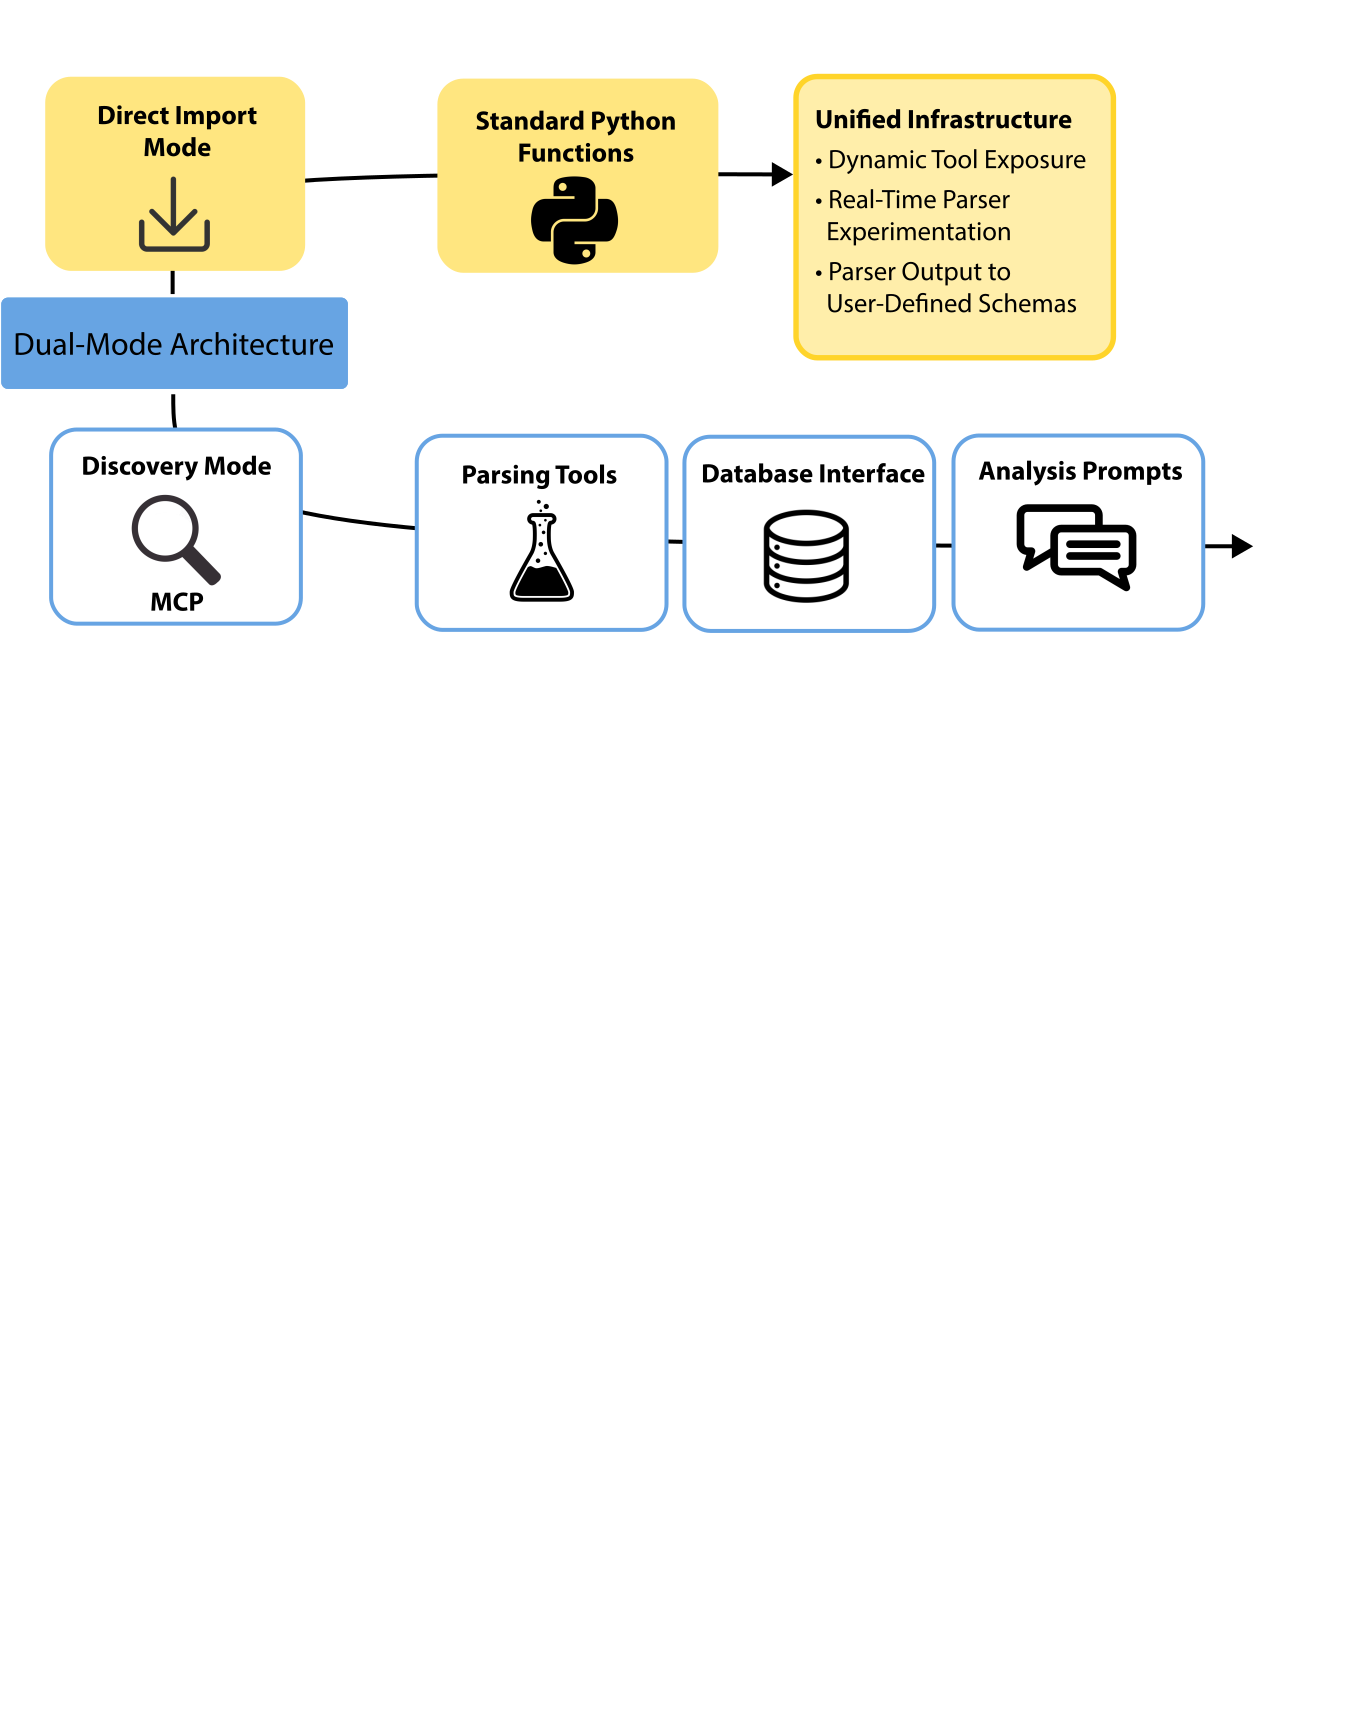
\includegraphics[width=0.5\linewidth]{figures/parse-patrol.png}
    \caption{
    \textbf{Parse-Patrol:}
    The dual-mode architecture allows for user queries via discovery mode and direct Python import mode for parsing big quantum chemistry software files properly.
    }
    \label{fig:parse-patrol}
\end{figure}

\section*{Future Work}

We will not tackle specific input formats in this project, therefore future work includes expanding the repository of supported parsers e.g. within the NOMAD\cite{nomad_lab,draxl2019nomad} and Materials Project\cite{Jain2013} frameworks, integrating coordination among multiple AI agents, and developing modular parsing functions optimized for specific chemistry subdomains.

